\section{Breadth First Search}

\subsection{200. Number of Islands}

\paragraph{\color{white} \colorbox{Mahogany}{Description}}
Given a 2d grid map of '1's (land) and '0's (water), count the number of islands. An island is surrounded by water and is formed by connecting adjacent lands horizontally or vertically. You may assume all four edges of the grid are all surrounded by water.

\paragraph{\color{white} \colorbox{OliveGreen}{Solution}}
\underline{Code Hints:}
\begin{itemize}
    \item BFS on a \textbf{tree} does not need to check whether the node has been visited. BFS on a \textbf{matrix} can use the matrix itself to check the visiting status of each element.
\end{itemize}

\subsection{279. Perfect Squares}

\paragraph{\color{white} \colorbox{Mahogany}{Description}}
Given a positive integer n, find the least number of perfect square numbers (for example, 1, 4, 9, 16, ...) which sum to n.

For example, given n = 12, return 3 because 12 = 4 + 4 + 4; given n = 13, return 2 because 13 = 4 + 9.

\paragraph{\color{white} \colorbox{OliveGreen}{Solution}}

\underline{Recursion, Recursion with Memoisation, DP, Static DP:}

$$T(i)=\min\{1+T(i - k^2)|k^2\leqslant i\}$$

\underline{Code Hints:}
\begin{itemize}
    \item Change recursion to dynamic programming: for $T(i)=f(T(j))$ where $j < i$, dynamic programming codes for $T(n)$ are
\begin{minted}[linenos]{cpp}
vector<int> dp(n + 1, ...);
for (int i = 0; i <= n; i++)
    dp[i] = f(dp[j]);
return dp[n];
\end{minted}
    \item Change dynamic programming to \textbf{static} dynamic programming:
\begin{minted}[linenos]{cpp}
static vector<int> dp = {...};
while (dp.size() < n + 1)
    dp.push_back(f(dp[j]));
return dp[n];
\end{minted}
\end{itemize}

\underline{BFS:}
\begin{figure}[ht]
    \centering
    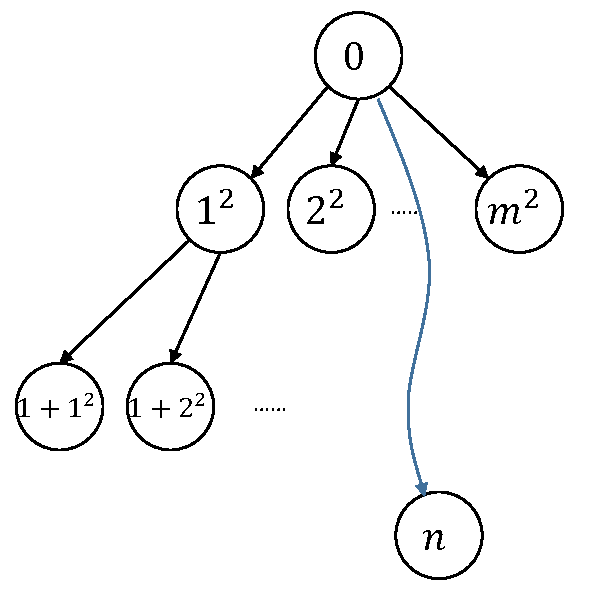
\includegraphics[width=6cm]{perfect_squares}
    \caption{Let's make $0$ as the root of the tree, the children of the $0$ root can be generated as $1^2,2^2,3^2,...,m^2$ where $m=\sqrt{n}$. Then, the children of the child node $1^2$ can be generated as $1^2+1^2,1^2+2^2,\cdots$, and the children of $2^2$ can be generated as $2^2+1^2,2^2+2^2,\cdots$. We apply BFS on the tree to find the first node which equals to the target $n$. The depth of this node is the least number of perfect square numbers which sum to $n$.}
    \label{fig:perfect_squares}
\end{figure}


\subsection{101. Symmetric Tree}

\paragraph{\color{white} \colorbox{Mahogany}{Description}}
Given a binary tree, check whether it is a mirror of itself (ie, symmetric around its center).

\paragraph{\color{white} \colorbox{OliveGreen}{Solution}}
\underline{Recursion:}
$$M(l, r)\gets v(l)=v(r)\wedge M(left(l), right(r))\wedge M(right(l), left(r))$$
$$S(r)\gets M(left(r), right(r))$$

\underline{Iteration (DFS):}
\underline{Code Hints:}
\begin{itemize}
    \item Use left-to-right traversal to the left subtree and right-to-left traversal to the right subtree in the same order (pre-order, in-order, or post-order).
\end{itemize}